\documentclass[wide,a4paper,titlepage,12pt] {article}
\usepackage{polski}
\usepackage[utf8]{inputenc}
\usepackage{listings}
\usepackage{slashbox}
\usepackage[table]{xcolor}
\usepackage{graphicx,pdflscape}
\usepackage{placeins}

\title{Projektowanie efektywnych algorytmów}
\author{Tymon Tobolski (181037)\\ Jacek Wieczorek (181043)}

% Title page layout (fold)
\makeatletter
\renewcommand{\maketitle}{
\begin{titlepage}
  \begin{center}
    \vspace*{3cm}
    \LARGE \@title \par
    \vspace{2cm}
    \textit{\small Autor:}\par
    \normalsize \@author\par \normalsize
    \vspace{3cm}
    \textit{\small Prowadzący:}\par
   Prof. dr hab. inż Adam Janiak \par
    \vspace{2cm}
    Wydział Elektroniki\\ III rok\\ Cz TN 13.15 - 15.00\par
    \vspace{4cm}
    \small \@date
  \end{center}
\end{titlepage}
}
\makeatother

\begin{document}
\maketitle
  \section{Cel projektu}
\paragraph{}
Celem projektu jest zaimplementowanie i przetestowanie metaheurystycznego algorytmu symulowanego wyżarzania dla problemu szeregowania zadań na jednym procesorze przy kryterium minimalizacji ważonej sumy opóźnień zadań.
  \section{Opis problemu}
{\bf Jednoprocesorowy problem szeregowania zadań przy kryterium
minimalizacji ważonej sumy opóźnień zadań.}
\paragraph{}
Danych jest $n$ zadań (o numerach od 1 do $n$), które mają być wykonane bez przerwań przez pojedynczy procesor, mogący wykonywać co najwyżej jedno zadanie jednocześnie.
Każde zadanie j jest dostępne do wykonania w chwili zero, do wykonania wymaga $p_{j} > 0$ jednostek czasu oraz ma określoną wagę (priorytet) $w_{j} > 0$ i oczekiwany termin zakończenia
wykonywania $d_{j} > 0$. Zadanie $j$ jest spóźnione, jeżeli zakończy się wykonywać po swoim terminie $d_{j}$, a miarą tego opóźnienia jest wielkość $T_{j} = max(0, C_{j} - d_{j} )$, gdzie $C_{j}$ jest terminem zakończenia
wykonywania zadania $j$. Problem polega na znalezieniu takiej kolejności wykonywania zadań (permutacji) aby zminimalizować kryterium $TWT = \Sigma_{j=1}^{n} w_{j} T_{j}$.
\section{Opis algorytmu}
\paragraph{}
Symulowane wyżarzanie to algorytm heurystyczny przeszukująy przestrzeń alternatywnych rozwiązań problemu w celu wyszukania rozwiązań najlepszych. Sposób działania algorytmu jest analogią do zjawiska wyżarzania w metalurgii.
\paragraph{}
Przebieg algorytmu :
\lstset{ %
    language=c++,                % choose the language of the code
    basicstyle=\scriptsize,       % the size of the fonts that are used for the code
    numbers=left,                   % where to put the line-numbers
    numberstyle=\scriptsize,      % the size of the fonts that are used for the line-numbers
    stepnumber=10,                   % the step between two line-numbers. If it's 1 each line 
                                    % will be numbered
    numbersep=9pt,                  % how far the line-numbers are from the code
    % backgroundcolor=\color{white},  % choose the background color. You must add \usepackage{color}
    showspaces=false,               % show spaces adding particular underscores
    showstringspaces=false,         % underline spaces within strings
    showtabs=false,                 % show tabs within strings adding particular underscores
    % frame=single,                 % adds a frame around the code
    % tabsize=2,                  % sets default tabsize to 2 spaces
    % captionpos=b,                   % sets the caption-position to bottom
    breaklines=true,                % sets automatic line breaking
    % breakatwhitespace=false,        % sets if automatic breaks should only happen at whitespace
    % title=\lstname,                 % show the filename of files included with \lstinputlisting;
                                    % also try caption instead of title
    % escapeinside={\%*}{*)},         % if you want to add a comment within your code
    % morekeywords={*,...}            % if you want to add more keywords to the set
    }
    \lstinputlisting{pseudokod.txt}
\paragraph{}
gdzie :
\begin{itemize}
  \item $S$ - funkcja generujaca nowy losowy stan na postawie podanego
  \item $F$ - funkcja celu/kosztu
  \item $P$ - prawdopodobieństwo przejścia do stanu o wyższym koszcie
  \item $T$ - funkcja czasu
\end{itemize}
\section{Implementacja}
\paragraph{}
Jezykiem implementacji algorytmu jest $Scala$ w wersji $2.9.1$ działająca na $JVM$. 
\paragraph{}
Algorytm oparty został na funkcji rekurencyjnej (rekurencja ogonowa) implementującej symulowane wyżarzanie. W celu bezpiecznego zrównoleglenia uruchamiania programy na wiele wątków i tym samym przyśpieszenia wyliczania skorzystaliśmy z programowania funkcyjnego.

\lstset{ %
    language=java,                % choose the language of the code
    basicstyle=\scriptsize,       % the size of the fonts that are used for the code
    numbers=left,                   % where to put the line-numbers
    numberstyle=\scriptsize,      % the size of the fonts that are used for the line-numbers
    stepnumber=10,                   % the step between two line-numbers. If it's 1 each line 
                                    % will be numbered
    numbersep=9pt,                  % how far the line-numbers are from the code
    % backgroundcolor=\color{white},  % choose the background color. You must add \usepackage{color}
    showspaces=false,               % show spaces adding particular underscores
    showstringspaces=false,         % underline spaces within strings
    showtabs=false,                 % show tabs within strings adding particular underscores
    % frame=single,                 % adds a frame around the code
    % tabsize=2,                  % sets default tabsize to 2 spaces
    % captionpos=b,                   % sets the caption-position to bottom
    breaklines=true,                % sets automatic line breaking
    % breakatwhitespace=false,        % sets if automatic breaks should only happen at whitespace
    % title=\lstname,                 % show the filename of files included with \lstinputlisting;
                                    % also try caption instead of title
    % escapeinside={\%*}{*)},         % if you want to add a comment within your code
    % morekeywords={*,...}            % if you want to add more keywords to the set
    }
    \lstinputlisting{sa.scala}

\newpage
\section{Testy}
\paragraph{}
Testy algorytmu symulowanego wyżarzania przeprowadzone zostały dla trzech zestawów testów o różnym rozmiarze porblemu $n$, każdy składający się ze 125 instancji. Parametry podstawowe jak $T_{min}$ i $T_{max}$ w przypadku każdego testu były takie same. Zmieniany natomiast był parametr $T_{d}$.
\paragraph{}
Jako wyniki testów przedstawiamy średni czas liczenia wszystkich instancji dla danego rozmiaru problemu - $\bar{t}$, a także średni błąd wzgledny  rozwiązań dla każdej instancji - $\bar{x}$. Według wzoru : \\
\begin{equation}
	\bar{t} = \frac{\Sigma_{j=1}^{n}\frac{\Sigma_{i=1}^{k}t_{i}}{k}}{n}
\end{equation}
\begin{equation}
	\bar{x} = \frac{\Sigma_{j=1}^{n}\frac{\Sigma_{i=1}^{k}x_{i}}{k}}{n}
\end{equation}
gdzie : \\
\begin{itemize}
  \item $k$ - ilość rozwiązań w instancji
  \item $n$ - ilość instancji danego problemu
\end{itemize}
\paragraph{}
Parametry niezmienne : 
\begin{itemize}
  \item $T_{min} = 0.01$
  \item $T_{max} = 100$
\end{itemize}
\newpage
\subsection{n = 40}
\begin{center}
    \begin{tabular}{|c|c|c|}
      \hline
       $T_{d}$ & Time & Difference \\ \hline
       0,99 & 5,78 & 27,41 \\ \hline
       0,999 & 46,26 & 2,52 \\ \hline
       0,9999 & 434,52 & 0,43 \\ \hline
  \end{tabular}
\end{center}

\begin{figure}[htbp]
  \begin{center}
         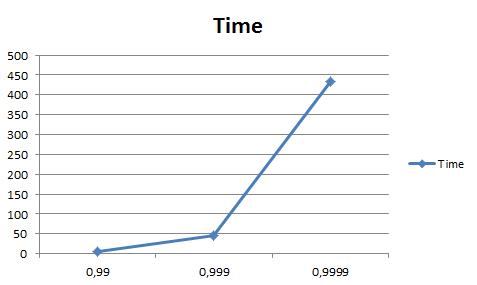
\includegraphics[scale=0.8]{time40.PNG}
         \caption{Czas rozwiązywania w zależności od parametru $T_d$}
  \end{center}
\end{figure}

\begin{figure}[htbp]
  \begin{center}
         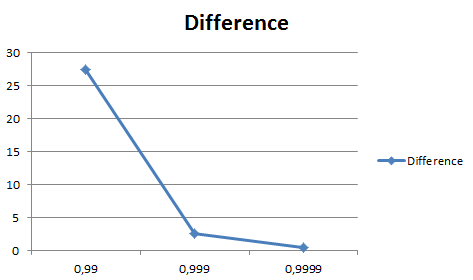
\includegraphics[scale=0.8]{diff40.PNG}
         \caption{Błąd względny rozwiązywania w zależności od parametru $T_d$}
  \end{center}
\end{figure}

\newpage
\subsection{n = 50}
\begin{center}
    \begin{tabular}{|c|c|c|}
      \hline
       $T_{d}$ & Time & Difference \\ \hline
       0,99 & 6,63 & 169,02 \\ \hline
       0,999 & 53,09 &8,47 \\ \hline
       0,9999 & 519,04 & 0,95 \\ \hline
  \end{tabular}
\end{center}

\begin{figure}[htbp]
  \begin{center}
         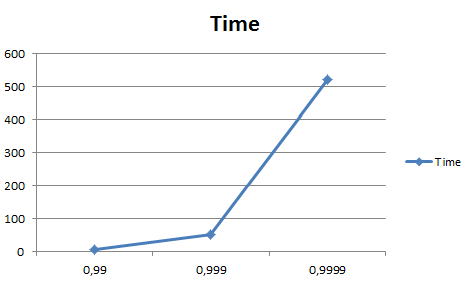
\includegraphics[scale=0.8]{time50.PNG}
         \caption{Czas rozwiązywania w zależności od parametru $T_d$}
  \end{center}
\end{figure}

\begin{figure}[htbp]
  \begin{center}
         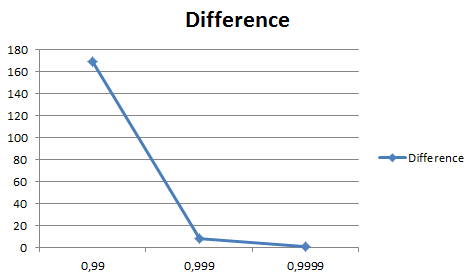
\includegraphics[scale=0.8]{diff50.PNG}
         \caption{Błąd względny rozwiązywania w zależności od parametru $T_d$}
  \end{center}
\end{figure}

\newpage
\subsection{n = 100}
\begin{center}
    \begin{tabular}{|c|c|c|}
      \hline
       $T_{d}$ & Time & Difference \\ \hline
       0,99 & 12,4 & 579,97 \\ \hline
       0,999 & 104,18 & 23,43 \\ \hline
       0,9999 & 990 & 3,42 \\ \hline
  \end{tabular}
\end{center}

\begin{figure}[htbp]
  \begin{center}
         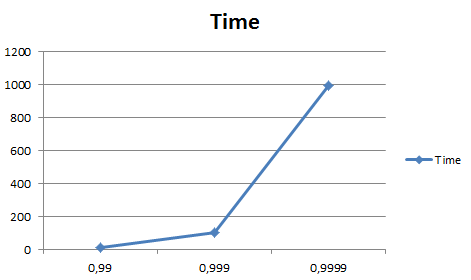
\includegraphics[scale=0.8]{time100.PNG}
         \caption{Czas rozwiązywania w zależności od parametru $T_d$}
  \end{center}
\end{figure}

\begin{figure}[htbp]
  \begin{center}
         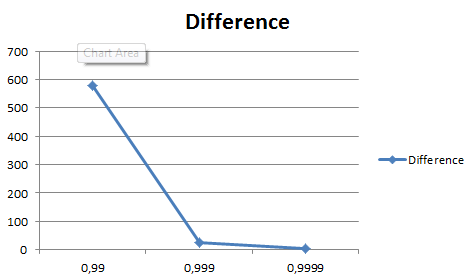
\includegraphics[scale=0.8]{diff100.PNG}
         \caption{Błąd względny rozwiązywania w zależności od parametru $T_d$}
  \end{center}
\end{figure}
\newpage
\subsection{Porównanie wszytskich zadań}
\begin{figure}[htbp]
  \begin{center}
         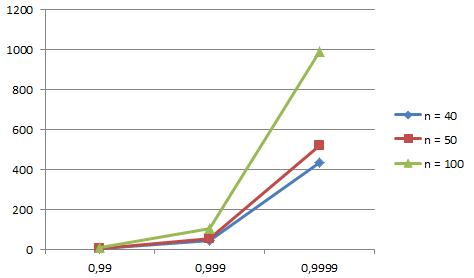
\includegraphics[scale=0.8]{complexTime.PNG}
         \caption{Czas rozwiązywania w zależności od parametru $T_d$}
  \end{center}
\end{figure}

\begin{figure}[htbp]
  \begin{center}
         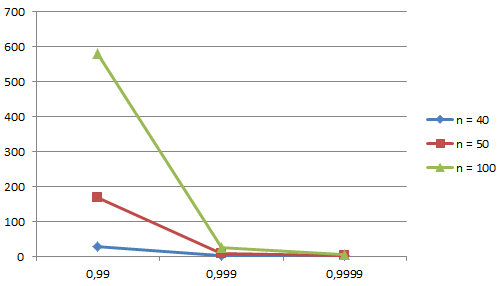
\includegraphics[scale=0.8]{complexDiff.PNG}
         \caption{Błąd względny rozwiązywania w zależności od parametru $T_d$}
  \end{center}
\end{figure}
\newpage
\section{Wnioski}
\paragraph{}
Analizując wyniki testów łatwo zauważyć, że rozmiar instancji ma znaczny wpływ na czas działania algorytmu. Pomimo tej samej liczby iteracji (dla ustalonego $T_d$ i zmiennego $n$) samego algorymu dużo czasu zajmuje obliczanie funkcji celu, która jest liniowo zależna od rozmiaru instancji. Na czas algorytmu ma również wpływ parametr $T_{d}$ określający jak szybko zmienia sie temperatura. Ilość iteracji algorytmu (zależna od parametru $T_d$, stałe $n$) ma również wpływ na jakość wyników. Im parametr $T_d$ jest większy, tym wynik dokładniejszy. Niestety zwiększa to ilość samych iteracji dla danego problemu : \\
\begin{center}
    \begin{tabular}{|c|c|}
      \hline
       $T_{d}$ & Ilość iteracji \\ \hline
       0,99 & 917 \\ \hline
       0,999 & 9206 \\ \hline
       0,9999 & 92099  \\ \hline
  \end{tabular}
\end{center}
Jak widać na wykresie dla $T_d$ = 0.99 i $n$ = 100 algorytm uzyskał średnią wzglądną róznicą od optymalnego wyniku na poziomie 500\%. Analizując poszczegąlne instancje błąd wzglądny wahal się od 10 do nawet 2500\%.
\paragraph{}
Algorytm symulowanego wyżarznia pozwala na znacznie szybsze wyznaczenie dokładnego lub zbliżonego do dokładnego rozwiązania niz przegląd zupełny. Wiąże się to jednak z koniecznością dobrania odpowiednich parametrów, co nie jest zadaniem łatwym. W miarę poprawy wyników poprzez dobierane parametry, wzrasta czas wykonania algorytmu. W celu obliczenia problemu, musimy odpowiedzieć sobie na pytanie, jak dokładne rozwiązanie nas interesuje i ile czasu możemy na nie poświęcić.  
\end{document}



